\section{Substitution Rule}\label{sec:SubRule}



Antiderivatives play a key role in the the process of evaluating definite integrals exactly.  In particular, the Fundamental Theorem of Calculus tells us that if $F$ is any antiderivative of $f$, then
$$\int_a^b f(x) \, dx = F(b) - F(a).$$
Furthermore, we realized that each elementary derivative rule leads to a corresponding elementary antiderivative (or indefinite integral), as summarized in Table~\ref{T:4.4.Act2}.  Thus, if we wish to evaluate an integral such as 
$$\int_0^1 \left(x^3 - \sqrt{x} + 5^x \right) \,dx,$$
it is straightforward to do so, since we can easily integrate $f(x) = x^3 - \sqrt{x} + 5^x.$ In particular, since a function $F$ whose derivative is $f$ is given by $F(x) = \frac{1}{4}x^4 - \frac{2}{3}x^{3/2} + \frac{1}{\ln(5)}5^x$, the Fundamental Theorem of Calculus tells us that
\begin{eqnarray*}
\int_0^1 \left(x^3 - \sqrt{x} + 5^x\right) \,dx & = & \left. \frac{1}{4}x^4 - \frac{2}{3}x^{3/2} + \frac{1}{\ln(5)}5^x\right|_0^1 \\
								& = & \left( \frac{1}{4}(1)^4 - \frac{2}{3}(1)^{3/2} + \frac{1}{\ln(5)}5^1 \right) - \left( \frac{1}{4}(0)^4 - \frac{2}{3}(0)^{3/2} + \frac{1}{\ln(5)}5^0 \right) \\
								& = & \frac{1}{4} - \frac{2}{3} + \frac{5}{\ln(5)} - \frac{1}{\ln(5)} \\
								& = & -\frac{5}{12} + \frac{4}{\ln(5)}.
\end{eqnarray*}
Because an algebraic formula for an antiderivative of $f$ enables us to evaluate the definite integral $\int_a^b f(x) \, dx$ exactly, we see that we have a natural interest in being able to find such algebraic antiderivatives.  Note that we emphasize \emph{algebraic} antiderivatives, as opposed to any antiderivative, since we know by the Second Fundamental Theorem of Calculus that $G(x) = \int_a^x f(t) \, dt$ is indeed an antiderivative of the given function $f$, but one that still involves a definite integral.  One of our main goals in this section is to develop understanding, in select circumstances, of how to ``undo'' the process of differentiation in order to find an algebraic antiderivative for a given function.


\subsection*{Reversing the Chain Rule: Substitution} 

It is usually straightforward to integrate a function of the form
$$h(x) = f(u(x)),$$
whenever $f$ is a familiar function whose antiderivative is known and $u(x)$ is a linear function.  For example, if we consider
$$h(x) = (5x-3)^6,$$
in this context the \textit{outer function} $f$ is $f(u) = u^6$, while the \textit{inner function} is $u(x) = 5x - 3$.  Since the antiderivative of $f$ is $F(u) = \frac{1}{7}u^7+C$, we 
see that the antiderivative of $h$ is
$$H(x) = \frac{1}{7} (5x-3)^7 \cdot \frac{1}{5} + C = \frac{1}{35} (5x-3)^7 + C.$$
The inclusion of the constant $\frac{1}{5}$ is essential precisely because the derivative of the inner function is $u'(x) = 5$.  Indeed, if we now compute $H'(x)$, we find by the Chain Rule (and Constant Multiple Rule) that
$$H'(x) = \frac{1}{35} \cdot 7(5x-3)^6 \cdot 5 = (5x-3)^6 = h(x),$$
and thus $H$ is indeed the general antiderivative of $h$.

Hence, in the special case where the outer function is familiar and the inner function is linear, we can antidifferentiate composite functions according to the following rule.


\begin{formulabox}[]{
If $h(x) = f(ax + b)$ and $F$ is a known algebraic antiderivative of $f$, then the general antiderivative of $h$ is given by
$$H(x) = \frac{1}{a} F(ax+b) + C.$$
}
\end{formulabox}

Of course, a natural question  arises: what happens when the inner function is not a linear function?  For example, can we find antiderivatives of such functions as 
$$g(x) = x e^{x^2} \ \mbox{and} \ h(x) = e^{x^2}?$$

It is important to explicitly remember that differentiation and antidifferentiation are essentially inverse processes; that they are not quite inverse processes is due to the $+C$ that arises when antidifferentiating.  This close relationship enables us to take any known derivative rule and translate it to a corresponding rule for an indefinite integral.  For example, since
$$\frac{d}{dx} \left[x^5\right] = 5x^4,$$
we can equivalently write
$$\int 5x^4 \, dx = x^5 + C.$$

Recall that the Chain Rule states that
$$\frac{d}{dx} \left[ f(g(x)) \right] = f'(g(x)) \cdot g'(x).$$
Restating this relationship in terms of an indefinite integral,
\begin{equation} \label{E:usubst}
\int f'(g(x)) g'(x) \, dx = f(g(x))+C.
\end{equation}
Hence, Equation~(\ref{E:usubst}) tells us that if we can take a given function and view its algebraic structure as $f'(g(x)) g'(x)$ for some appropriate choices of $f$ and $g$, then we can antidifferentiate the function by reversing the Chain Rule.  It is especially notable that both $g(x)$ and $g'(x)$ appear in the form of $f'(g(x)) g'(x)$; we will sometimes say that we seek to \emph{identify a function-derivative pair}\index{function-derivative pair} when trying to apply the rule in Equation~(\ref{E:usubst}).

For example: Find
$$\int 2x\cos(x^2)\,dx.$$
This is not a ``simple'' derivative, but a little thought reveals that
it must have come from an application of the chain rule. Multiplied
on the ``outside'' is $2x$, which is the derivative of the ``inside''
function $\ds x^2$. Checking:
$${d\over dx}\sin(x^2)  = \cos(x^2){d\over dx}x^2 = 2x\cos(x^2),$$
so 
$$\int 2x\cos(x^2)\,dx=\sin(x^2)+C .$$

In the situation where we can identify a function-derivative pair, we will introduce a new variable $u$ to represent the function $g(x)$.  Observing that with $u = g(x)$, it follows in Leibniz notation that $\frac{du}{dx} = g'(x)$, so that in terms of differentials\footnote{If we recall from the definition of the derivative that $\frac{du}{dx} \approx \frac{\triangle{u}}{\triangle{x}}$ and use the fact that $\frac{du}{dx} = g'(x)$, then we see that $g'(x) \approx \frac{\triangle{u}}{\triangle{x}}$.  Solving for $\triangle u$, $\triangle u \approx g'(x) \triangle x$.  It is this last relationship that, when expressed in ``differential'' notation enables us to write $du = g'(x) \, dx$ in the change of variable formula.}, $du = g'(x)\, dx$.  Now converting the indefinite integral of interest to a new one in terms of $u$, we have  
$$\int f'(g(x)) g'(x) \, dx = \int f'(u) \,du.$$
Provided that $f'$ is an elementary function whose antiderivative is known, we can now easily evaluate the indefinite integral in $u$, and then go on to determine the desired overall antiderivative of $f'(g(x)) g'(x)$.  We call this process \emph{$u$-substitution}. 

To summarize: If we suspect that a given function is the derivative of
another via the chain rule, we let $u$ denote a likely candidate for
the inner function, then translate the given function so that it is
written entirely in terms of $u$, with no $x$ remaining in the
expression. If we can integrate this new function of $u$, then the
antiderivative of the original function is obtained by replacing $u$
by the equivalent expression in $x$.

\begin{theorem}{$ u $-Substitution Rule for Indefinite Integrals}{SubstitutionRule}
If $u=g(x)$ is a differentiable function whose range is an interval $I$ and $f$ is continuous on $I$, then
$$\int f(g(x))g'(x)\,dx=\int f(u)\,du.$$
\end{theorem}

Even in simple cases you may prefer to use this mechanical procedure,
since it often helps to avoid silly mistakes. For example, consider
again this simple problem:
$$\int 2x\cos(x^2)\,dx.$$
Let $\ds u=x^2$, then $du/dx = 2x$ or $du = 2x\,dx$. Since we have exactly 
$2x\,dx$ in the original integral, we can replace it by $du$:
$$\int 2x\cos(x^2)\,dx=\int \cos u\,du=\sin u +C = \sin(x^2)+C.$$
This is not the only way to do the algebra, and typically there are
many paths to the correct answer. Another possibility, for example,
is: Since $du/dx = 2x$, $dx=du/2x$, and then the integral becomes
$$\int 2x\cos(x^2)\,dx=\int 2x\cos u\,{du\over 2x}=\int \cos u\,du.$$
The important thing to remember is that you must eliminate all
instances of the original variable $x$.

\begin{example}{Substitution Rule}{usub}\label{usub}
Evaluate the indefinite integral
$$\int x^3 \cdot \sin (7x^4 + 3) \, dx$$
and check the result by differentiating.
\end{example}

\begin{solution} 
We can make two key algebraic observations stand regarding the integrand, $x^3 \cdot \sin (7x^4 + 3)$.  First, $\sin (7x^4 + 3)$ is a composite function; as such, we know we'll need a more sophisticated approach to antidifferentiating.  Second, $x^3$ is almost the derivative of $(7x^4 + 3)$; the only issue is a missing constant.  Thus, $x^3$ and $(7x^4 + 3)$ are nearly a function-derivative pair.  Furthermore, we know the antiderivative of $f(u) = \sin(u)$.  The combination of these observations suggests that we can evaluate the given indefinite integral by reversing the chain rule through $u$-substitution.

Letting $u$ represent the inner function of the composite function $\sin (7x^4 + 3)$, we have
$$u = 7x^4 + 3,$$
and thus $\frac{du}{dx} = 28x^3.$  In differential notation, it follows that $du = 28x^3 \, dx$, and thus $x^3 \, dx = \frac{1}{28} \, du$.  We make this last observation because the original indefinite integral may now be written 
$$\int \sin (7x^4 + 3) \cdot x^3 \, dx,$$
and so by substituting the expressions in $u$ for $x$ (specifically $u$ for $7x^4 + 3$ and $\frac{1}{28} \, du$ for $x^3 \, dx$), it follows that
$$\int \sin (7x^4 + 3) \cdot x^3 \, dx = \int \sin(u) \cdot \frac{1}{28} \, du.$$
Now we may evaluate the original integral by first evaluating the easier integral in $u$, followed by replacing $u$ by the expression $7x^4 + 3$.  Doing so, we find
\begin{eqnarray*}
\int \sin (7x^4 + 3) \cdot x^3 \, dx & = & \int \sin(u) \cdot \frac{1}{28} \, du \\
						& = & \frac{1}{28} \int \sin(u) \, du \\
						& = & \frac{1}{28} (-\cos(u)) + C \\
						& = & -\frac{1}{28} \cos(7x^4 + 3) + C.
\end{eqnarray*}
To check our work, we observe by the Chain Rule that
$$\frac{d}{dx} \left[ -\frac{1}{28}\cos(7x^4 + 3) + C \right] = -\frac{1}{28} \cdot (-1)\sin(7x^4 + 3) \cdot 28x^3 = \sin(7x^4 + 3) \cdot x^3,$$
which is indeed the original integrand.
\end{solution}

An essential observation about our work in Example~\ref{usub}  is that the $u$-substitution only worked because the function multiplying $\sin (7x^4 + 3)$ was $x^3$.  If instead that function was $x^2$ or $x^4$, the substitution process may not (and likely would not) have worked.  This is one of the primary challenges of antidifferentiation: slight changes in the integrand make tremendous differences.  For instance, we can use $u$-substitution with $u = x^2$ and $du = 2xdx$ to find that
\begin{eqnarray*}
\int xe^{x^2} \, dx & = & \int e^u \cdot \frac{1}{2} \, du \\
			& = & \frac{1}{2} \int e^u \, du \\
			& = & \frac{1}{2} e^u + C \\
			& = & \frac{1}{2} e^{x^2} + C.
\end{eqnarray*}
If, however, we consider the similar indefinite integral
$$\int e^{x^2} \, dx,$$
the missing $x$ to multiply $e^{x^2}$ makes the $u$-substitution $u = x^2$ no longer possible.  Hence, part of the lesson of $u$-substitution is just how specialized the process is: it only applies to situations where, up to a missing constant, the integrand that is present is the result of applying the Chain Rule to a different, related function.



\begin{example}{Substitution Rule}{SubstitutionRuleex}
Evaluate $\ds\int(ax+b)^n\,dx$, assuming $a,b$ are
constants, $a\not=0$, and $n$ is a positive integer.
\end{example}

\begin{solution} 
We let $u=ax+b$ so $du=a\,dx$ or $dx=du/a$. Then
$$
  \int(ax+b)^n\,dx=\int {1\over a} u^n\,du={1\over a(n+1)}u^{n+1}+C=
  {1\over a(n+1)}(ax+b)^{n+1}+C.
$$
\end{solution}

\begin{example}{Substitution Rule}{SubstitutionRulex}
Evaluate $\ds\int \sin(ax+b)\,dx$, assuming that $a$ and $b$ are
constants and $a\not=0$.
\end{example}

\begin{solution} 
Again we let $u=ax+b$ so $du=a\,dx$ or $dx=du/a$. Then
$$
  \int\sin(ax+b)\,dx=\int {1\over a} \sin u\,du={1\over a}(-\cos u)+C=
-{1\over a}\cos(ax+b)+C.
$$
\end{solution}

\begin{formulabox}[Strategy for Substitution Rule]
A general strategy to follow is:
\begin{enumerate}\setlength{\itemsep}{0 in}
\item Choose a possible $u=u(x)$. \dfont{Tip:} Choose a substitution $u$ so that its derivate also appears in the integral (up to a constant).
\item Calculate $du=u'(x)~dx$.
\item Either replace $u'(x)~dx$ by $du$, or replace $dx$ by $\ds{\frac{du}{u'(x)}}$, and cancel.
\item Write the rest of the integrand in terms of $u$. If this is not possible, the substitution will not work: You must go back to step 1.
\item Find the indefinite integral. (Again, if this is not possible, try a different substitution, or a different method).
\item Rewrite the result in terms of $x$.
\end{enumerate}
\end{formulabox}

\begin{example}{Substitution}{Substitution}
Evaluate the following integral: $\ds\int \frac{2x}{\sqrt{1-4x^2}}\,dx.$
\end{example}

\begin{solution} 
We try the substitution:
$$u=1-4x^2.$$
Then,
$$du=-8x~dx$$
In the numerator we have $2x~dx$, so rewriting the differential gives:
$$-\frac{1}{4}du=2x~dx.$$
Then the integral is:
\begin{eqnarray*}
\int \frac{2x}{\sqrt{1-4x^2}}\,dx&=&\int \left(1-4x^2\right)^{-1/2}(2x~dx)\\
\\
&=&\int u^{-1/2}\left(-\frac{1}{4}du\right)\\
\\
&=&\left(\frac{-1}{4}\right)\frac{u^{1/2}}{1/2}+C\\
\\
&=&-\frac{\sqrt{1-4x^2}}{2}+C
\end{eqnarray*}
\end{solution}



\begin{example}{Substitution}{Substitution}
Evaluate the following integral: $\ds\int \sech^2(7t-3)\ dt$
\end{example}

\begin{solution} 
 We employ substitution, with $u = 7t-3$ and $du = 7dt$. We have:
$$ \int \sech^2 (7t-3)\ dt=  \frac17 \int \sech^2 (u)\ du= \frac17\tanh (u) + C = \frac17\tanh (7t-3) + C.$$
\end{solution}





\begin{example}{Substitution}{Substitution2}
Evaluate the following integral: $\ds\int \cos x(\sin x)^5\,dx.$
\end{example}

\begin{solution} 
In this question we will let $u=\sin x$.
Then,
$$du=\cos x~dx.$$
Thus, the integral becomes:
\begin{eqnarray*}
\int \cos x(\sin x)^5\,dx&=&\int u^5\,du\\
\\
&=&\frac{u^6}{6}+C\\
\\
&=&\frac{(\sin x)^6}{6}+C
\end{eqnarray*}
\end{solution}

\begin{example}{Substitution}{Substitution3}
Evaluate the following integral:
$\ds\int \frac{\cos(\sqrt x)}{\sqrt x}\,dx.$
%\vspace{-0.5cm}
\end{example}

\begin{solution} 
We use the substitution:
$$u=x^{1/2}.$$
Then,
$$du=\frac{1}{2}x^{-1/2}dx.$$
Rewriting the differential we get:
$$2~du=\frac{1}{\sqrt x}~dx.$$
The integral becomes:
\begin{eqnarray*}
\int \frac{\cos(\sqrt x)}{\sqrt x}\,dx&=&2\int \cos u\,du\\
\\
&=&2\sin u+C\\
\\
&=&2\sin(\sqrt x)+C
\end{eqnarray*}
\end{solution}



%\begin{example}{Substitution with Inverse Trigonometric Functions}{Substitution with Inverse Trigonometric Functions}
%From items \ref{invsin} and \ref{invtan} in  Theorem \ref{thm:indef_alg} and the method of substitution with $ u=\frac{x}{a} $ where $ a>0 $ (try it!), we get the following:
%\[
%\int \frac{1}{x^2+a^2}=\frac1a\arctan\left(\frac{x}{a}\right)+C \text{ and } \int \frac{1}{\sqrt{a^2-x^2}}\; dx = \arcsin\left(\frac{x}{a}\right)+C
%\] 

%\end{example}

\begin{example}{Integrating by substitution}{ex_sub10}
{
Evaluate $\ds \int \sin x\cos x\ dx$.
}
\end{example}

\begin{solution}
{There is not a composition of function here to exploit; rather, just a product of functions. Do not be afraid to experiment; when given an integral to evaluate, it is often beneficial to think ``If I let $u$ be \textit{this}, then $du$ must be \textit{that} \ldots'' and see if this helps simplify the integral at all.

In this example, let's set $u = \sin x$. Then $du = \cos x\ dx$, which we have as part of the integrand! The substitution becomes very straightforward:
		\begin{align*}
		\int \sin x\cos x\ dx &=	\int u\ du \\
											&= \frac12u^2+ C \\
											&= \frac12\sin^2 x + C.
		\end{align*}
One would do well to ask ``What would happen if we let $u = \cos x$?'' The result is just as easy to find, yet looks very different. The challenge to the reader is to evaluate the integral letting $u = \cos x$ and discover why the answer is the same, yet looks different.
}
\end{solution}



Our examples so far have required ``basic substitution.'' The next example demonstrates how substitutions can be made that often strike the new learner as being ``nonstandard.''\\

%\enlargethispage{\baselineskip}


\begin{example}{Substitution}{Substitution4}
Evaluate the following integral:
$\ds\int 2x^3\sqrt{x^2+1}\,dx.$
%\vspace{-0.5cm}
\end{example}

\begin{solution} 
This problem is a little bit different than the previous ones.
It makes sense to let:
$$u=x^2+1,$$
then
$$du=2x~dx.$$
Making this substitution gives:
\begin{eqnarray*}
\int 2x^3\sqrt{x^2+1}\,dx&=&\int x^2\sqrt{x^2+1}(2x)\,dx\\
\\
&=&\int x^2u^{1/2}\,du\\
\end{eqnarray*}
This is a problem because our integrals can't have a mixture of two variables in them.
Usually this means we chose our $u$ incorrectly.
However, in this case we can eliminate the remaining $x$'s from our integral by using:
$$u=x^2+1\quad\to\quad x^2=u-1.$$
We get:
\begin{eqnarray*}
\int x^2u^{1/2}\,du&=&\int (u-1)u^{1/2}\,du\\
\\
&=&\int u^{3/2}-u^{1/2}\,du\\
\\
&=&\frac{2}{5}u^{5/2}-\frac{2}{3}u^{3/2}+C\\
\\
&=&\frac{2}{5}(x^2+1)^{5/2}-\frac{2}{3}(x^2+1)^{3/2}+C
\end{eqnarray*}
\end{solution}


\begin{example}{Integrating by substitution}{ex_sub4}
Evaluate $\ds\int x\sqrt{x+3}\ dx$.
\end{example}
\begin{solution}
{Recognizing the composition of functions, set $u = x+3$. Then $du = dx$, giving what seems initially to be a simple substitution. But at this stage, we have:
	$$\int x\sqrt{x+3}\ dx = \int x\sqrt{u}\ du.$$
We cannot evaluate an integral that has both an $x$ and an $u$ in it. We need to convert the $x$ to an expression involving just $u$.

Since we set $u = x+3$, we can also state that $u-3 = x$. Thus we can replace $x$ in the integrand with $u-3$. It will also be helpful to rewrite $\sqrt{u}$ as $u^\frac12$.
\begin{align*}
		\int x\sqrt{x+3} \ dx &= \int (u-3)u^\frac12\ du \\
											&= \int \big(u^\frac32 - 3u^\frac12\big) \ du \\
											&= \frac25u^\frac52 - 2u^\frac32 + C \\
											&= \frac25(x+3)^\frac52 - 2(x+3)^\frac32 + C.
\end{align*}
Checking your work is always a good idea. In this particular case, some algebra will be needed to make one's answer match the integrand in the original problem.
}
\end{solution}


\begin{example}{Integrating by substitution}{ex_sub5}
Evaluate $\ds \int \frac{1}{x\ln x}\ dx$.
\end{example}

\begin{solution}
{This is another example where there does not seem to be an obvious composition of functions. The line of thinking used in Example \ref{exa:ex_sub4} is useful here: choose something for $u$ and consider what this implies $du$ must be. If $u$ can be chosen such that $du$ also appears in the integrand, then we have chosen well.

Choosing $u = 1/x$ makes $du = -1/x^2\ dx$; that does not seem helpful. However, setting $u = \ln x$ makes $du = 1/x\ dx$, which is part of the integrand. Thus:
\begin{align*}
	\int \frac1{x\ln x}\ dx 	&=	\int \frac{1}{\underbrace{\ln x}_{1/u}}\underbrace{\frac1x\ dx}_{du} \\
												&= \int \frac1u\ du \\
												&= \ln |u| + C \\
												&= \ln | \ln x| + C.
\end{align*}
The final answer is interesting; the natural log of the natural log. Take the derivative to confirm this answer is indeed correct.
}
\end{solution}

\subsection{Integrals Involving Trigonometric Functions}

Section \ref{sec:Powers of trigonometric functions} delves deeper into integrals of a variety of trigonometric functions; here we use substitution to establish a foundation that we will build upon. 

The next three examples will help fill in some missing pieces of our antiderivative knowledge. We know the antiderivatives of the sine and cosine functions; what about the other standard functions tangent, cotangent, secant and cosecant? We discover these next.\\

\begin{example}{Integration by substitution: antiderivatives of $\tan x$}{ex_sub6}
Evaluate $\ds \int \tan x\ dx.$
\end{example}

\begin{solution}
{The previous paragraph established that we did not know the antiderivatives of tangent, hence we must assume that we have learned something in this section that  can help us evaluate this indefinite integral. 

%\enlargethispage{\baselineskip}
Rewrite $\tan x$ as $\sin x/\cos x$. While the presence of a composition of functions may not be immediately obvious, recognize that $\cos x$ is ``inside'' the $1/x$ function. Therefore, we see if setting $u = \cos x$ returns usable results. We have that $du = -\sin x\ dx$, hence $-du = \sin x\ dx$. We can integrate:
\begin{align*}
		\int \tan x \ dx &= \int \frac{\sin x}{\cos x}\ dx \\
							&= \int \frac1{\underbrace{\cos x}_u}\underbrace{\sin x\ dx}_{-du} \\
							&= \int \frac {-1}u \ du\\
							&= -\ln |u| + C \\
							&= -\ln |\cos x| + C.
\end{align*}
Some texts prefer to bring the $-1$ inside the logarithm as a power of $\cos x$, as in:
\begin{align*}
-\ln |\cos x| + C &= \ln |(\cos x)^{-1}| + C\\
			&= \ln \left| \frac{1}{\cos x}\right| + C\\
			&= \ln |\sec x| + C.
\end{align*}
Thus the result they give is $\int \tan x \ dx = \ln|\sec x| + C$. These two answers are equivalent.
}\\

\end{solution}

\begin{example}{Integrating by substitution: antiderivatives of $\sec x$}{ex_sub7}
Evaluate $\ds\int \sec x\ dx$.
\end{example}

%\enlargethispage{2\baselineskip}

\begin{solution}
{This example employs a wonderful trick: multiply the integrand by ``1'' so that we see how to integrate more clearly. In this case, we write ``1'' as
$$1 = \frac{\sec x + \tan x}{\sec x + \tan x}.$$
This may seem like it came out of left field, but it works beautifully. Consider:
\begin{align*}
			\int \sec x\ dx	&=	\int \sec x\cdot \frac{\sec x + \tan x}{\sec x + \tan x}\ dx \\
							&= \int \frac{\sec^2 x + \sec x\tan x}{\sec x + \tan x}\ dx.\\
\intertext{Now let $u = \sec x+\tan x$; this means $du = (\sec x\tan x+ \sec^2 x)\ dx$, which is our numerator. Thus:}
						&= \int \frac{du}{u} \\
						&= \ln |u| + C \\
						&= \ln |\sec x+\tan x| + C.
\end{align*}
\vskip -\baselineskip
}
\end{solution}

%\clearpage


We can use similar techniques to those used in Examples \ref{ex_sub6} and \ref{ex_sub7} to find antiderivatives of $\cot x$ and $\csc x$ (which the reader can explore in the exercises.) We summarize our results here.

\begin{theorem}{Antiderivatives of Trigonometric Functions}{triganti}
{\begin{minipage}{.45\textwidth}\small\index{integration!of trig. functions}
	\begin{enumerate}
	\item		$\ds \int \sin x \ dx = -\cos x +C$
	\item		$\ds\int \cos x\ dx = \sin x + C$
	\item		$\ds \int \tan x\ dx = -\ln|\cos x|+C$
\end{enumerate}
\end{minipage}
\begin{minipage}{.55\textwidth}\small
	\begin{enumerate}\addtocounter{enumi}{3}
	\item		$\ds \int \csc x \ dx = -\ln|\csc x+\cot x| +C$
	\item		$\ds\int \sec x\ dx = \ln|\sec x+\tan x| + C$
	\item		$\ds \int \cot x\ dx = \ln|\sin x|+C$
\end{enumerate}
\end{minipage}
}
\end{theorem}



We explore one more common trigonometric integral.\\

\begin{example}{Integration by substitution: powers of $\cos x$ and $\sin x$}{ex_sub8}
{
Evaluate $\ds \int \cos^2x\ dx$.}
\end{example}

\begin{solution}
{We have a composition of functions as $\cos^2x = \big(\cos x\big)^2$. 
%with $\cos x$ inside the $x^2$ function. 
However, setting $u = \cos x$ means $du = -\sin x\ dx$, which we do not have in the integral. Another technique is needed.

The process we'll employ is to use a Power Reducing formula for $\cos^2x$ (perhaps consult the back of this text for this formula), which states 
	$$\cos ^2x = \frac{1+\cos(2x)}{2}.$$
	The right hand side of this equation is not difficult to integrate. We have:
\begin{align*}
	\int \cos^2x\ dx &= \int \frac{1+\cos(2x)}2\ dx \\
									&=	\int \left( \frac12 + \frac12\cos(2x)\right)\ dx. \\
\intertext{Now use Key Idea \ref{idea:linearsub}:}
									&= \frac12x + \frac12\frac{\sin(2x)}{2} + C \rule[-10pt]{0pt}{5pt}\\
									&= \frac12x + \frac{\sin(2x)}4 + C.
\end{align*}
We'll make significant use of this power--reducing technique in future sections.
}\\
\end{solution}



\subsection{ Simplifying the Integrand}

It is common to be reluctant to manipulate the integrand of an integral; at first, our grasp of integration is tenuous and one may think that working with the integrand will improperly change the results. Integration by substitution works using a different logic: as long as \textit{equality} is maintained, the integrand can be manipulated so that its \textit{form} is easier to deal with. The next two examples demonstrate common ways in which using algebra first makes the integration easier to perform.\\

%\enlargethispage{2\baselineskip}

\begin{example}{Integration by substitution: simplifying first}{ex_sub9}
{
Evaluate $\ds\int \frac{x^3+4x^2+8x+5}{x^2+2x+1}\ dx$.}
\end{example}

\begin{solution}
{One may try to start by setting $u$ equal to either the numerator or denominator; in each instance, the result is not workable. 

When dealing with rational functions (i.e., quotients made up of polynomial functions), it is an almost universal rule that everything works better when the degree of the numerator is less than the degree of the denominator. Hence we use polynomial division.

We skip the specifics of the steps, but note that when $x^2+2x+1$ is divided into $x^3+4x^2+8x+5$, it goes in $x+2$ times with a remainder of $3x+3$. Thus 
	$$\frac{x^3+4x^2+8x+5}{x^2+2x+1} = x+2 + \frac{3x+3}{x^2+2x+1}.$$
Integrating $x+2$ is simple. The fraction can be integrated by setting $u = x^2+2x+1$, giving $du = (2x+2)\ dx$. This is very similar to the numerator. Note that $du/2 = (x+1)\ dx$ and then consider the following:
\begin{align*}
\int \frac{x^3+4x^2+8x+5}{x^2+2x+1}\ dx & = \int \left(x+2 + \frac{3x+3}{x^2+2x+1}\right)\ dx  \rule[-13pt]{0pt}{5pt} \\
					&= \int (x+2)\ dx + \int \frac{3(x+1)}{x^2+2x+1}\ dx  \rule[-13pt]{0pt}{5pt}\\
					& = \frac12x^2+2x+C_1 + \int \frac{3}{u}\frac{du}{2}  \rule[-13pt]{0pt}{5pt}\\
					&= \frac12x^2+2x+C_1 + \frac32\ln|u| + C_2 \rule[-13pt]{0pt}{5pt}\\
					&= \frac12x^2+2x+\frac32\ln|x^2+2x+1| + C.
\end{align*}
In some ways, we ``lucked out'' in that after dividing, substitution was able to be done. In later sections we'll develop techniques for handling rational functions where substitution is not directly feasible.
}\\
\end{solution}


\begin{example}{Integration by alternate methods}{ex_sub11}
{
Evaluate $\ds\int \frac{x^2+2x+3}{\sqrt{x}}\ dx$ with, and without, substitution.}
\end{example}


\begin{solution}
{We already know how to integrate this particular example. Rewrite $\sqrt{x}$ as $x^\frac12$ and simplify the fraction:
	$$ \frac{x^2+2x+3}{x^{1/2}} = x^\frac32 + 2x^\frac12 + 3x^{-\frac12}.$$
We can now integrate using the Power Rule:
\begin{align*}
	\int \frac{x^2+2x+3}{x^{1/2}}\ dx &= \int\left(x^\frac32 + 2x^\frac12 + 3x^{-\frac12}\right)\ dx\\
						&=	\frac25x^\frac52 + \frac43x^\frac32 + 6x^\frac12 + C
\end{align*}
This is a perfectly fine approach. We demonstrate how this can also be solved using substitution as its implementation is rather clever.

Let $u = \sqrt{x} = x^\frac12$; therefore 
		$$du = \frac12x^{-\frac12}dx = \frac{1}{2\sqrt{x}}\ dx \quad \Rightarrow \quad 2du = \frac{1}{\sqrt{x}}\ dx.$$
		
This gives us $\ds \int \frac{x^2+2x+3}{\sqrt{x}}\ dx = \int (x^2+2x+3)\cdot2\ du$. What are we to do with the other $x$ terms? Since $u = x^\frac12$, $u^2 = x$, etc. We can then replace $x^2$ and $x$ with appropriate powers of $u$. We thus have
\begin{align*}
\int \frac{x^2+2x+3}{\sqrt{x}}\ dx &= \int (x^2+2x+3)\cdot2\ du\\
											&= \int 2(u^4 + 2u^2 + 3)\ du \\
											&= \frac25u^5 + \frac43u^3 + 6u + C \\
											&= \frac25x^\frac52 + \frac43x^\frac32 + 6x^\frac12+C,
\end{align*}
which is obviously the same answer we obtained before. In this situation, substitution is arguably more work than our other method. The fantastic thing is that it works. It demonstrates how flexible integration is.
}
\end{solution}




\subsection{Substitution and Inverse Trigonometric Functions}

%In Section \ref{sec:deriv_inverse_function} 
When studying derivatives of inverse functions, we learned that $$\frac{d}{dx}\big(\tan^{-1}x\big) = \frac{1}{1+x^2}.$$ Applying the Chain Rule to this is not difficult; for instance, $$\frac{d}{dx}\big(\tan^{-1}5x\big) = \frac{5}{1+25x^2}.$$ We now explore how Substitution can be used to ``undo'' certain derivatives that are the result of the Chain Rule applied to Inverse Trigonometric functions. We begin with an example.\\

\begin{example}{Integrating by substitution: inverse trigonometric functions}{ex_subst14}
{
Evaluate $\ds \int \frac{1}{25+x^2}\ dx$.}
\end{example}

\begin{solution}
{The integrand looks similar to the derivative of the arctangent function. Note:
\begin{align*}
\frac{1}{25+x^2} &= \frac{1}{25(1+\frac{x^2}{25})}\\
							&= \frac{1}{25(1+\left(\frac{x}{5}\right)^2)} \\
							&= \frac{1}{25}\frac{1}{1+\left(\frac{x}{5}\right)^2}\ .
\end{align*}
Thus $$\int\frac{1}{25+x^2}\ dx = \frac{1}{25}\int \frac{1}{1+\left(\frac{x}{5}\right)^2}\ dx.$$ This can be integrated using Substitution. Set $u = x/5$, hence $du = dx/5$ or $dx=5du$. Thus
\begin{align*}
\int\frac{1}{25+x^2}\ dx &= \frac{1}{25}\int \frac{1}{1+\left(\frac{x}{5}\right)^2}\ dx \\
										&= \frac15\int \frac{1}{1+u^2}\ du \\
										&= \frac15\tan^{-1}u + C \\
										&= \frac15\tan^{-1}\left(\frac x5\right)+C
\end{align*}
\vskip -\baselineskip
}
\end{solution}



Example \ref{exa:ex_subst14} demonstrates a general technique that can be applied to other integrands that result in inverse trigonometric functions. The results are summarized here.


\begin{theorem}{Integrals Involving Inverse Trigonomentric Functions}{int_inverse_trig}
{Let $a>0$.
%\noindent\begin{minipage}[t]{.5\linewidth}
\begin{enumerate}
\item		$\ds \int \frac{1}{a^2+x^2}\ dx = \frac1a\tan^{-1}\left(\frac{x}{a}\right) + C$
%\addtocounter{enumi}{1}
\item		$\ds \int \frac{1}{\sqrt{a^2-x^2}}\ dx = \sin^{-1}\left(\frac{x}{a}\right)+C$
%\end{enumerate}
%\end{minipage}
%\begin{minipage}[t]{.5\linewidth}
%\begin{enumerate}\addtocounter{enumi}{1}
\item		$\ds \int \frac{1}{x\sqrt{x^2-a^2}}\ dx = \frac1a\sec^{-1}\left(\frac{|x|}{a}\right)+C$
\end{enumerate}
%\end{minipage}
}
\end{theorem}


Let's practice using Theorem \ref{thm:int_inverse_trig}.\\

\begin{example}{Integrating by substitution: inverse trigonometric functions}{ex_subst15}
{Evaluate the given indefinite integrals.
$$\int \frac{1}{9+x^2}\ dx,\quad \int \frac{1}{x\sqrt{x^2-\frac{1}{100}}}\ dx\quad \text{ and }\quad  \int \frac{1}{\sqrt{5-x^2}}\ dx.$$
}
\end{example}

\begin{solution}
{Each can be answered using a straightforward application of Theorem \ref{thm:int_inverse_trig}.\\

$\ds \int \frac{1}{9+x^2}\ dx = \frac13\tan^{-1} \frac x3 + C$, as $a = 3$.\vskip 10pt

$\ds \int  \frac{1}{x\sqrt{x^2-\frac{1}{100}}}\ dx = 10\sec^{-1}10x + C$, as $a = \frac1{10}$.\vskip 10pt

$\ds \int \frac{1}{\sqrt{5-x^2}} = \sin^{-1}\frac{x}{\sqrt{5}}+C$, as $a = \sqrt{5}$.\\
}
\end{solution}



\enlargethispage{2\baselineskip}
Most applications of Theorem \ref{thm:int_inverse_trig} are not as straightforward. The next examples show some common integrals that can still be approached with this theorem.\\

\begin{example}{Integrating by substitution: completing the square}{ex_subst16}
{Evaluate $\ds \int\frac{1}{x^2-4x+13}\ dx$.}
\end{example}

\begin{solution}
{Initially, this integral seems to have nothing in common with the integrals in Theorem \ref{thm:int_inverse_trig}. As it lacks a square root, it almost certainly is not related to arcsine or arcsecant. It is, however, related to the arctangent function.

We see this by \textit{completing the square} in the denominator. We give a brief reminder of the process here. 

Start with a quadratic with a leading coefficient of 1. It will have the form of $x^2 + bx + c$. Take 1/2 of $b$, square it, and add/subtract it back into the expression. I.e., 
\begin{align*} 
x^2+bx+ c &= \underbrace{x^2 + bx + \frac{b^2}4}_{(x+b/2)^2} - \frac{b^2}4 + c\\
   &= \left(x+\frac b2\right)^2 + c-\frac{b^2}4
\end{align*}
In our example, we take half of $-4$ and square it, getting $4$. We add/subtract it into the denominator as follows:

\begin{align*}
\frac{1}{x^2-4x+13} &= \frac{1}{\underbrace{x^2-4x+4}_{(x-2)^2}-4+13}\\
				&=\frac{1}{(x-2)^2 + 9}
\end{align*}
We can now integrate this using the arctangent rule. Technically, we need to substitute first with $u=x-2$, but we omit this step here. Thus we have 
$$ \int \frac{1}{x^2-4x+13}\ dx = \int \frac{1}{(x-2)^2+9}\ dx = \frac13\tan^{-1}\frac{x-2}{3}+C.$$
\vskip -\baselineskip
}
\end{solution}


\begin{example}{Integrals requiring multiple methods}{ex_subst17}
{
Evaluate $\ds \int \frac{4-x}{\sqrt{16-x^2}}\ dx$.}
\end{example}

\begin{solution}
{This integral requires two different methods to evaluate it. We get to those methods by splitting up the integral: 
$$ \int \frac{4-x}{\sqrt{16-x^2}}\ dx = \int \frac{4}{\sqrt{16-x^2}}\ dx - \int \frac{x}{\sqrt{16-x^2}}\ dx.$$
The first integral is handled using a straightforward application of Theorem \ref{thm:int_inverse_trig}; the second integral is handled by substitution, with $u = 16-x^2$. We handle each separately.

$\ds \int \frac{4}{\sqrt{16-x^2}}\ dx = 4\sin^{-1}\frac{x}{4} + C$.
\vskip 10pt

$\ds \int\frac{x}{\sqrt{16-x^2}}\ dx$: Set $u = 16-x^2$, so $du = -2xdx$ and $xdx = -du/2$. We have 
\begin{align*}
\int\frac{x}{\sqrt{16-x^2}}\ dx &= \int\frac{-du/2}{\sqrt{u}}\\
				&= -\frac12\int \frac{1}{\sqrt{u}}\ du \\
				&= - \sqrt{u} + C\\
				&= -\sqrt{16-x^2} + C.
\end{align*}
Combining these together, we have 
$$ \int \frac{4-x}{\sqrt{16-x^2}}\ dx = 4\sin^{-1}\frac x4 + \sqrt{16-x^2}+C.$$
}
\end{solution}






% % % % % % % % % % % % % % % % % % % % % % % % % % % % % % % % % %

This section has focused on evaluating indefinite integrals as we are learning a new technique for finding antiderivatives. However, much of the time integration is used in the context of a definite integral. Definite integrals that require substitution can be calculated using the following workflow:

\begin{enumerate}
\item		Start with a definite integral $\ds \int_a^b f(x)\ dx$ that requires substitution.
\item		Ignore the bounds; use substitution to evaluate $\ds \int f(x)\ dx$ and find an antiderivative $F(x)$.
\item		Evaluate $F(x)$ at the bounds; that is, evaluate $F(x)\Big|_a^b = F(b) - F(a)$.
\end{enumerate}
This workflow works fine, but substitution offers an alternative that is powerful and amazing (and a little time saving).  The next example shows how to use the Substitution Rule when dealing with definite integrals.

\begin{example}{Substitution Rule}{SubstitutionRuledefex}
Evaluate $\ds\int_2^4 x\sin(x^2)\,dx$. 
\end{example}

\begin{solution} 
First we compute the
antiderivative, then evaluate the integral.
Let $\ds u=x^2$, so $du=2x\,dx$ or $x\,dx=du/2$. Then
$$
  \int x\sin(x^2)\,dx=\int {1\over 2} \sin u\,du={1\over 2}(-\cos u)+C=
  -{1\over 2}\cos(x^2)+C.
$$
Now
$$
  \int_2^4 x\sin(x^2)\,dx=\left.-{1\over 2}\cos(x^2)\right|_2^4
  =-{1\over 2}\cos(16)+{1\over 2}\cos(4).
$$
A somewhat neater alternative to this method is to change the original
limits to match the variable $u$. Since $\ds u=x^2$, when $x=2$, $u=4$,
and when $x=4$, $u=16$. So we can do this:
$$
  \int_2^4 x\sin(x^2)\,dx=
  \int_4^{16} {1\over 2} \sin u\,du=\left.-{1\over 2}(\cos u)\right|_4^{16}
  =-{1\over 2}\cos(16)+{1\over 2}\cos(4).
$$
An incorrect, and dangerous, alternative is something like this:
$$
  \int_2^4 x\sin(x^2)\,dx=\int_2^4 {1\over 2} \sin u\,du=
  \left.-{1\over 2}\cos (u)\right|_2^4=
  \left.-{1\over 2}\cos(x^2)\right|_2^4=-{1\over 2}\cos(16)+{1\over
  2}\cos(4).
$$
This is incorrect because $\ds\int_2^4 {1\over 2} \sin u\,du$
means that $u$ takes on values between 2 and 4, which is wrong. It
is dangerous, because it is very easy to get to 
the point $\ds\left.-{1\over 2}\cos (u)\right|_2^4$ and forget to substitute
$\ds x^2$ back in for $u$, thus getting the incorrect answer
$\ds -{1\over 2}\cos(4)+{1\over 2}\cos(2)$. An acceptable alternative is something like:
$$ 
  \int_2^4 x\sin(x^2)\,dx=\int_{x=2}^{x=4} {1\over 2} \sin u\,du=
  \left.-{1\over 2}\cos (u)\right|_{x=2}^{x=4}=
  \left.-{1\over 2}\cos(x^2)\right|_2^4=-{\cos(16)\over 2}+{\cos(4)\over2}.
$$
\end{solution}

\subsection{Substitution and Definite Integrals}

The following theorem states how the bounds of a definite integral can be changed as the substitution is performed.

\begin{theorem}{Substitution Rule for Definite Integrals}{SubstitutionRuledef}
If $g'$ is continuous on $[a,b]$ and $f$ is continuous on the range of $u=g(x)$, then
$$\int_a^b f(g(x))g'(x)\,dx=\int_{g(a)}^{g(b)}f(u)\,du.$$
\end{theorem}



In effect, Theorem \ref{thm:SubstitutionRuledef} states that once you convert to integrating with respect to $u$, you do not need to switch back to evaluating with respect to $x$. A few examples will help one understand.\\

\begin{example}{Definite integrals and substitution: changing the bounds}{ex_sub12}
{
Evaluate $\ds\int_0^2 \cos(3x-1)\ dx$ using Theorem \ref{thm:SubstitutionRuledef}.}
\end{example}

\begin{solution}
{Observing the composition of functions, let $u=3x-1$, hence $du = 3dx$. As $3dx$ does not appear in the integrand, divide the latter equation by 3 to get $du/3 = dx$. 

By setting $u = 3x-1$, we are implicitly stating that $g(x) = 3x-1$. Theorem \ref{thm:SubstitutionRuledef} states that the new lower bound is $g(0) = -1$; the new upper bound is $g(2) = 5$. We now evaluate the definite integral:
\begin{align*}
\int_1^2 \cos(3x-1) \ dx &=	\int_{-1}^5 \cos u \frac{du}{3} \\
								&= \frac{1}{3} \sin u\Big|_{-1}^5 \\
								&= \frac{1}{3}\big(\sin 5- \sin (-1)\big)\approx -0.039.
								%&\approx -0.039.
\end{align*}
Notice how once we converted the integral to be in terms of $u$, we never went back to using $x$.




\begin{figure}
\centering
\begin{subfigure}{.5\textwidth}
  \centering
  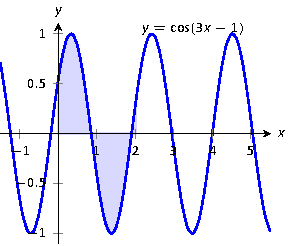
\includegraphics[width=.8\textwidth]{figures/figsubst12a}
  \caption{}
  \label{fig:sub1}
\end{subfigure}%
\begin{subfigure}{.5\textwidth}
  \centering
  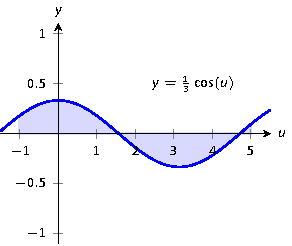
\includegraphics[width=.8\textwidth]{figures/figsubst12b}
  \caption{}
  \label{fig:sub2}
\end{subfigure}
\caption{Graphing the areas defined by the definite integrals of Example \ref{exa:ex_sub12}. \label{fig:subst12}}
\label{fig:test}
\end{figure}



%\begin{figure}
%\centering
%
%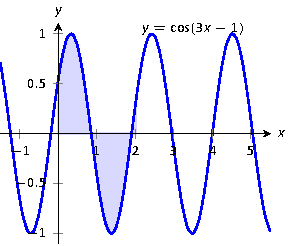
\includegraphics[width=0.7\linewidth]{figures/figsubst12a}
%
%\caption{Graphing the areas defined by the definite integrals in Example \ref{exa:ex_sub12}}
%\label{fig:figsubst12a}
%\end{figure}
%
%
%\mtable{.7}{Graphing the areas defined by the definite integrals of Example \ref{exa:ex_sub12}.}{fig:subst12}{\begin{tabular}{ccc}
%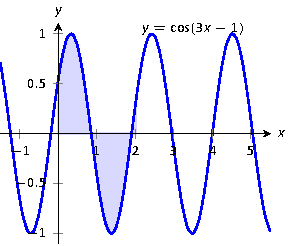
\includegraphics{figures/figsubst12a} & &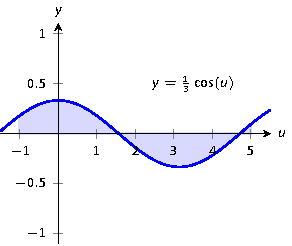
\includegraphics{figures/figsubst12b}\\
%(a) & & (b)
%\end{tabular}


The graphs in Figure \ref{fig:subst12} tell more of the story. In (a) the area defined by the original integrand is shaded, whereas in (b) the area defined by the new integrand is shaded. In this particular situation, the areas look very similar; the new region is ``shorter'' but ``wider,'' giving the same area.
}\\
\end{solution}


\begin{example}{Definite integrals and substitution: changing the bounds}{ex_subst13}
{
Evaluate $\ds \int_0^{\pi/2} \sin x \cos x\ dx$ using Theorem \ref{thm:SubstitutionRuledef}.
}
\end{example}

\begin{solution}
{We saw the corresponding indefinite integral in Example \ref{exa:ex_sub10}. In that example we set $u = \sin x$ but stated that we could have let $u = \cos x$. For variety, we do the latter here.

Let $u = g(x) = \cos x$, giving $du = -\sin x\ dx$ and hence $\sin x\ dx = -du$. The new upper bound is $g(\pi/2) = 0$; the new lower bound is $g(0) = 1$. Note how the lower bound is actually larger than the upper bound now. We have
\begin{align*}
	\int_0^{\pi/2} \sin x\cos x\ dx &= \int_1^0 -u\ du \quad \text{\scriptsize (switch bounds \& change sign)}\\%&= \int_1^0u\ (-1)du\\
											%&= \int_1^0 -u\ du \quad \text{\scriptsize (switch bounds \& change sign)}\\
											&=	\int_0^1 u\ du\\
											&= \frac12u^2\Big|_0^1= 1/2.%\\
											%&= 1/2.
\end{align*}
In Figure \ref{fig:subst13} we have again graphed the two regions defined by our definite integrals. Unlike the previous example, they bear no resemblance to each other. However, Theorem \ref{thm:SubstitutionRuledef} guarantees that they have the same area.


\begin{figure}
\centering
\begin{subfigure}{.5\textwidth}
  \centering
  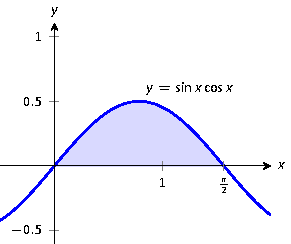
\includegraphics[width=.8\linewidth]{figures/figsubst13a}
  \caption{}
  \label{fig:sub1}
\end{subfigure}%
\begin{subfigure}{.5\textwidth}
  \centering
  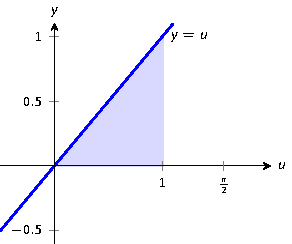
\includegraphics[width=.8\linewidth]{figures/figsubst13b}
  \caption{}
  \label{fig:sub2}
\end{subfigure}
\caption{Graphing the areas defined by the definite integrals of Example \ref{exa:ex_subst13}. \label{fig:subst13}}
\label{fig:test}
\end{figure}

%%\ifthenelse{\boolean{longpage}}
%%{% if longpage
%\mtable{.3}{Graphing the areas defined by the definite integrals of Example \ref{ex_subst13}.}{fig:subst13}{\begin{tabular}{ccc}
%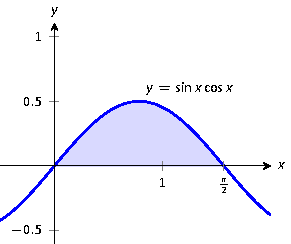
\includegraphics{figures/figsubst13a} & &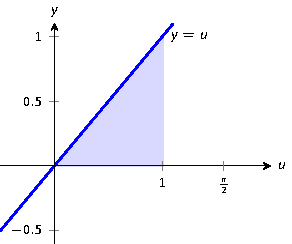
\includegraphics{figures/figsubst13b}\\
%(a) & & (b)
%\end{tabular}
%
%} %ends \mtable
%}% ends if longpage
%{% not longpage
%\mtable{.32}{Graphing the areas defined by the definite integrals of Example \ref{ex_subst13}.}{fig:subst13}{\begin{tabular}{c}
%\myincludegraphics{figures/figsubst13a} \\ (a) \\ \myincludegraphics{figures/figsubst13b}\\
%(b)
%\end{tabular}
%}% ends figure
%}% ends if not longpage 
%\vskip-\baselineskip
}
\end{solution}


\begin{example}{Substitution Rule}{SubstitutionRuledef2}
Evaluate $\ds\int_{1/4}^{1/2}{\cos(\pi t)\over\sin^2(\pi t)}\,dt$. 
\end{example}

\begin{solution} 
Let $u=\sin(\pi t)$ so $du=\pi\cos(\pi t)\,dt$ or $du/\pi=\cos(\pi
t)\,dt$.
We change the limits to $\ds \sin(\pi/4)=\sqrt2/2$ and 
$\sin(\pi/2)=1$.
Then
$$
  \int_{1/4}^{1/2}{\cos(\pi t)\over\sin^2(\pi t)}\,dt=
  \int_{\sqrt2/2}^{1}{1\over \pi}{1\over u^2}\,du=
  \int_{\sqrt2/2}^{1} {1\over \pi}u^{-2}\,du=
  \left.{1\over \pi}{u^{-1}\over -1}\right|_{\sqrt2/2}^{1}=
  -{1\over\pi}+{\sqrt2\over\pi}.
$$
\end{solution}

The following theorem sometimes allows us to greatly simplify the calculations of integrals, by exploiting their symmetry.

\begin{theorem}{Integrals of Symmetric Functions}{symm_integrals}
Suppose $f$ is continuous on $[-a, a]$.
\begin{enumerate}
\item  If $f$ is  even  (that is,  {$f(-x) = f(x)$}), then $\displaystyle  { \int\limits_{-a}^a f(x) \ dx} = 2  {\int\limits_0^a f(x) \ dx}$.
\item  If $f$ is  {odd} (that is,  {$f(-x) = -f(x)$}), then $\displaystyle   {\int\limits_{-a}^a f(x) \  dx }=  {\int\limits_{0}^a f(x) \ dx}+  {\int\limits_{-a}^0 f(x) \ dx}= 0$.
\end{enumerate}
\end{theorem}


\begin{proof}
Since the definite integral is additive with respect to the interval of integration, we have
\[
\int_{-a}^{a} f(x) \; dx = \int_{-a}^{0} f(x) \; dx + \int_{0}^{a} f(x) \; dx =\star
\]
Substitute $ u=-x $ in the first integral to get 
\[
\star = \int_{ a}^{0} f(-u) \; -du + \int_{0}^{a} f(x) \; dx = \int_{ 0}^{a} f(-u) \; du + \int_{0}^{a} f(x) \; dx 
\]
Since $ u $ is simply a "dummy variable" we can replace it with $ x $ to get
\[
\star = \int_{ 0}^{a} f(-x) \; dx + \int_{0}^{a} f(x) \; dx = \int_{0}^{a} f(x) + f(-x) \; dx
\]
If $ f $ is even, then $ f(-x)=f(x) $, and   $ f $ is odd then $ f(x)+f(-x)=0 $ giving the equations in the theorem.
\end{proof}


\begin{figure}
\centering
\begin{subfigure}{.5\textwidth}
  \begin{tikzpicture}[/pgf/declare function={f= x^2+1;}]
    \begin{axis}[
      axis lines=middle,
       xtick       = {-2,0,2},
      xticklabels = {$-a$,$0$,$a$},
       ytick       = {},
       yticklabels = {},
      samples     = 160,
      domain      = -2:2,
      xmin = -2, xmax = 2,
      ymin = 0, ymax = 5,
    ]
    \addplot[name path=poly, black, thick, mark=none, ] {f};
     \addplot [draw=none,name path=B] {0};     % “fictional” curve
  %  \addplot[name path=line, gray, no markers, line width=1pt] {3};
   \addplot [green!60] fill between[of = poly and B,soft clip={domain=-2:2}]; % filling
    %\addplot [red!60] fill between[of = poly and B,soft clip={domain=2:4.2}]; % filling
    ];
    %% Choosing the coordinates manually is annoying:
    \node at (axis cs:-1,1) {$A_1$};
    \node at (axis cs:1,1) {$A_2$};
  \end{axis}
  \end{tikzpicture}
  \caption{Even symmetry, $ A_1=A_2$}
  \label{fig:symm1}
\end{subfigure}%
\begin{subfigure}{.5\textwidth}
\begin{tikzpicture}[/pgf/declare function={f=x^3;}]
  \begin{axis}[
      axis lines=middle,
      xtick       = {-2,0,2},
          xticklabels = {$-a$,$0$,$a$},
           ytick       = {},
          yticklabels = {},
      samples     = 160,
      domain      = -2:2,
      xmin = -2, xmax = 2,
      ymin = -8, ymax = 8,
    ]
  \addplot[name path=poly, black, thick, mark=none, ] {f};
   \addplot [draw=none,name path=B] {0};     % “fictional” curve
%  \addplot[name path=line, gray, no markers, line width=1pt] {3};
 \addplot [green!60] fill between[of = poly and B,soft clip={domain=0:2}]; % filling
  \addplot [red!60] fill between[of = poly and B,soft clip={domain=-2:0}]; % filling
  ];
  %% Choosing the coordinates manually is annoying:
  \node at (axis cs:-1.5,-1) {$A_1$};
  \node at (axis cs:1.5,1) {$A_2$};
\end{axis}
\end{tikzpicture}
\caption{Odd symmetry, $ A_1=-A_2$.}
  \label{fig:symm2}
\end{subfigure}
\label{fig:symm_integral}
\end{figure}

\begin{example}{Odd Symmetry and Integrals}{symm-integral1}
Use properties of integrals to evaluate $\displaystyle \int_{-3}^{3}1-x^4 {d}{x}$
\end{example}

\begin{solution}
Since $ 1-x^4 $ is an odd function, that is, if $ f(x)=1-x^4 $, then $ f(-x) = 1-(-x)^4=1-x^4=f(x)$. So by symmetry (Theorem \ref{thm:symm_integrals}) we have
\[
\int_{-3}^{3}1-x^4 {d}{x}=2\int_{0}^{3}1-x^4 {d}{x}= 2\left(x-\frac{x^5}{5}\right|+0^3=2\left(3-\frac{243}{5} \right)
= -\frac{456}{5}\]
\end{solution}


\begin{example}{Even Symmetry and Integrals}{symm-integral2}
Use properties of integrals to evaluate $\displaystyle{{{\int_{{-{5}}}^{{5}}}{\left(\frac{\sin(x)}{x^2+1} \right)}{d}{x}}}
$
\end{example}

\begin{solution}
Since $ sin(x) $ is an odd function, and $ x^2+1 $ is an even function, the quotient of the two is odd.  That is, if $ f(x)= \frac{\sin(x)}{x^2+1}   $, then $ f(-x) =  \frac{\sin(-x)}{(-x)^2+1}  = \frac{-\sin(x)}{x^2+1} = -f(x) $. So by symmetry (Theorem \ref{thm:symm_integrals}) we have
\[
\int_{-5}^{5}{\left(\frac{\sin(x)}{x^2+1} \right)}{d}{x}=0
\]
\end{solution}


Integration by substitution is a powerful and useful integration technique. Section \ref{sec:Parts} introduces another technique, called Integration by Parts. As substitution ``undoes'' the Chain Rule, integration by parts ``undoes'' the Product Rule. Together, these two techniques provide a strong foundation on which most other integration techniques are based.



%%%%%%%%%%%%%%%%%%%%%%%%%%%%%%%%%%%%%%%%%%%%%%%%%
\Opensolutionfile{solutions}[ex]
\section*{Exercises for Section \ref{sec:SubRule}}

\begin{enumialphparenastyle}

Find the following indefinite and definite integrals.

%%%%%%%%%%
\begin{ex}
 $\ds\int (1-t)^9\,dt$
\begin{sol}
 $\ds -(1-t)^{10}/10+C$
\end{sol}
\end{ex}

%%%%%%%%%%
\begin{ex}
 $\ds\int (x^2+1)^2\,dx$
\begin{sol}
 $\ds x^5/5+2x^3/3+x+C$
\end{sol}
\end{ex}

%%%%%%%%%%
\begin{ex}
 $\ds\int x(x^2+1)^{100}\,dx$
\begin{sol}
 $\ds (x^2+1)^{101}/202+C$
\end{sol}
\end{ex}

%%%%%%%%%%
\begin{ex}
 $\ds\int {1\over\root 3 \of {1-5t}}\,dt$ 
\begin{sol}
 $\ds -3(1-5t)^{2/3}/10+C$
\end{sol}
\end{ex}

%%%%%%%%%%
\begin{ex}
 $\ds\int \sin^3x\cos x\,dx$
\begin{sol}
 $\ds (\sin^4x)/4+C$
\end{sol}
\end{ex}

%%%%%%%%%%
\begin{ex}
 $\ds\int x\sqrt{100-x^2}\,dx$
\begin{sol}
 $\ds -(100-x^2)^{3/2}/3+C$
\end{sol}
\end{ex}

%%%%%%%%%%
\begin{ex}
 $\ds\int {x^2\over\sqrt{1-x^3}}\,dx$
\begin{sol}
 $\ds \ds -2\sqrt{1-x^3}/3+C$
\end{sol}
\end{ex}

%%%%%%%%%%
\begin{ex}
 $\ds\int \cos(\pi t)\cos\bigl(\sin(\pi t)\bigr)\,dt$
\begin{sol}
 $\ds \sin(\sin\pi t)/\pi+C$
\end{sol}
\end{ex}

%%%%%%%%%%
\begin{ex}
 $\ds\int {\sin x\over\cos^3 x}\,dx$
\begin{sol}
 $\ds \ds 1/(2\cos^2 x)=(1/2)\sec^2x+C$
\end{sol}
\end{ex}

%%%%%%%%%%
\begin{ex}
 $\ds\int\tan x\,dx$
\begin{sol}
 $-\ln|\cos x|+C$
\end{sol}
\end{ex}

%%%%%%%%%%
\begin{ex}
  $\ds\int_0^\pi\sin^5(3x)\cos(3x)\,dx$
\begin{sol}
 $0$
\end{sol}
\end{ex}

%%%%%%%%%%
\begin{ex}
 $\ds\int\sec^2x\tan x\,dx$
\begin{sol}
 $\ds \tan^2(x)/2+C$
\end{sol}
\end{ex}

%%%%%%%%%%
\begin{ex}
 $\ds\int_0^{\sqrt{\pi}/2} x\sec^2(x^2)\tan(x^2)\,dx$
\begin{sol}
 $1/4$
\end{sol}
\end{ex}

%%%%%%%%%%
\begin{ex}
 $\ds\int {\sin(\tan x)\over\cos^2x}\,dx$
\begin{sol}
 $-\cos(\tan x)+C$
\end{sol}
\end{ex}

%%%%%%%%%%
\begin{ex}
 $\ds\int_3^4 {1\over(3x-7)^2}\,dx$
\begin{sol}
 $1/10$
\end{sol}
\end{ex}

%%%%%%%%%%
\begin{ex}
 $\ds\int_0^{\pi/6}(\cos^2x - \sin^2x)\,dx$
\begin{sol}
 $\ds \sqrt3/4$
\end{sol}
\end{ex}

%%%%%%%%%%
\begin{ex}
 $\ds\int {6x\over(x^2 - 7)^{1/9}}\,dx$
\begin{sol}
 $\ds (27/8)(x^2-7)^{8/9}$
\end{sol}
\end{ex}

%%%%%%%%%%
\begin{ex}
 $\ds\int_{-1}^1 (2x^3-1)(x^4-2x)^6\,dx$
\begin{sol}
 $\ds -(3^7+1)/14$
\end{sol}
\end{ex}

%%%%%%%%%%
\begin{ex}
 $\ds\int_{-1}^1 \sin^7 x\,dx$
\begin{sol}
 $0$
\end{sol}
\end{ex}

%%%%%%%%%%
\begin{ex}
 $\ds\int f(x) f'(x)\,dx$ 
\begin{sol}
 $\ds f(x)^2/2$
\end{sol}
\end{ex}

\end{enumialphparenastyle}